\chapter{Introduction}
\pagenumbering{arabic} 
\setcounter{page}{1} 

Despite more than a century of active biology research, many biological systems lack good computational models.
Computational models are useful if they accurately capture how the underlying biological system behaves.
When these models are faithful to the underlying biology, experiments can be run \textit{in silico} instead of \textit{in vivo}, speeding up the pace of research.
Moreover, the best computational models are useful not only as biology simulators, but also as facilitators of new hypotheses.
Computational biology models should both help researchers improve their understanding of the modeled system and expose novel insights into the underlying biology.

Biological systems are complex and can be examined at various levels of abstraction.
For example, one model could use a physical description of a cell to predict its shape as it grows.
A different model could use -omic data---genomic, transcriptomic, and metabolomic measurements---to model the production of compounds that allow for cellular growth.
My efforts focus on modeling the metabolism of a biological system to help biologists better understand what reactions are occurring in that system.

The goal of this work is to provide a metabolic model of a Cell-Free Protein Synthesis (CFPS) system that is useful for biologists working with \gls{cfps} systems.
To that end, I introduce \gls{sys}, an end-to-end system that produces metabolic models for \gls{cfps} systems from experimental data.
\gls{sys} learns which reactions are most important for a given cell-free system and produces a reduced metabolic model that fits the experimental data.
These reduced models are produced through the use of a Variational Autoencoder (\gls{vae}) on top of a common metabolic modeling technique called Flux Balance Analysis (\gls{fba}).
In order to incorporate experimental data into the model, I also introduce a new \gls{vae} loss function based on correlation that I call a Corr-VAE.
The Corr-VAE perturbs the latent space of a \gls{vae} to better fit the experimental data.
%TODO: fix sentence
\gls{sys} can be used by biologists to navigate the parameter space of different starting conditions, cope with batch variation, and gain a deeper understand of the composition of cell-free systems.

\begin{figure}[t!]
\begin{center}
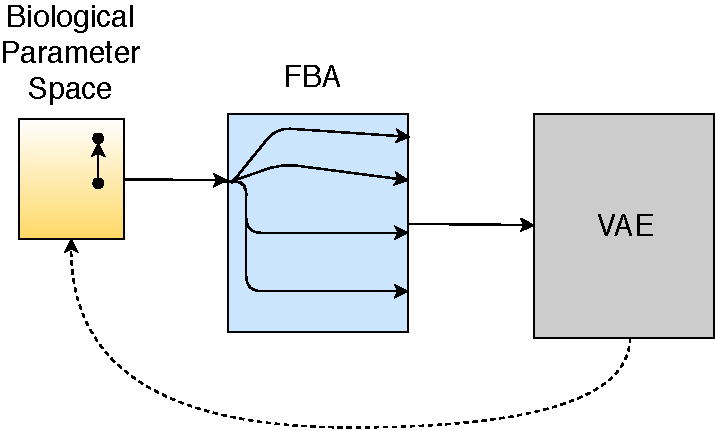
\includegraphics[width=\textwidth]{figs/FBA_Amplifier.pdf}
\end{center}
\caption[High-level idea behind \gls{sys}]{High-level idea behind \gls{sys}.
Small changes in the parameter space are amplified across many different fluxes in a \gls{fba} model.
A \gls{vae} can help elucidate how the changes in the fluxes in the \gls{fba} model reflect the changes in the parameter space. 
}
\label{fig:fba_amp}
\end{figure}

\textbf{Metabolic models}

Metabolism is defined as all of the chemical reactions that occur within an entity---usually an organism or a cell---in order to sustain its life and growth.
Biologists are interested in understanding how different parts of metabolism function, as metabolic reactions are the end result of the other biological process of interest (e.g. transcription and translation).
While ongoing work continues to develop a more robust understanding of metabolism, recent advances have begun to explore applications that involve manipulating the metabolism. 
Metabolic engineering has the potential to create novel advances in medicine and energy production such as increased bioproduction of the antimalarial drug artemisin~\cite{keasling2012synthetic}.
Metabolic models are an important tool for metabolic engineers because they can be used to predict how the phenotype of an organism will respond to manipulation.

Many metabolic models represent the chemical reactions in a system with a mathematical representation of the reaction coefficients.
Individual reactions are denoted as equations in these models.
Mathematical constraints are placed on these reactions based on an understanding of the biological pathways they represent.
Models of this type are collected under the heading of \gls{cobra} models~\cite{schellenberger2011quantitative} and are very common in the metabolic engineering community~\cite{orth2010flux}.
One of the most popular constraint-based metabolic models is \gls{fba}.
It has been used in hundreds of different works to model metabolism~\cite{feist2008growing}.
These applications range from optimizing metabolic pathways~\cite{almaas2004global} to investigating gene networks~\cite{shlomi2007genome}.
\gls{fba} is based on a genome-scale metabolic models (\glspl{gem}) reconstructed from the genome of an organism of interest.
However, these \glspl{gem} describe living organisms, not cell-free systems, so typical \gls{fba} models cannot be applied out of the box to a cell-free system.

In addition, since metabolism is a heterogenous mixture of reactions, small changes in the parameter space can lead to large changes in the metabolic output of a system.
The parameter space for \gls{cfps} systems primarily consists of final concentrations of energy substrates.
Current models are unable to explain how changes in the concentration of a certain reactant will affect the output of a \gls{cfps} system.
Even using a modeling technique such as \gls{fba} will not solve this issue because \gls{fba} acts as a non-linear amplifier on small changes in the parameter space.
The use of a dimensionality reduction technique such as a \gls{vae} can help explain how the changes in the original parameter space are reflected in the output of a \gls{fba} model.
Figure \ref{fig:fba_amp} demonstrates this idea, a key motivation behind the creation of \gls{sys}.

Building this type of learning system requires datasets that explore across a biologically relevant parameter space.
These datasets are not common, so this dissertation required extensive experimental work in order to generate data that could be used to learn a model.
I will be also be releasing the \gls{cfps} datasets I generated to aid with further modeling work of \gls{cfps} systems.
Additionally, performing both the experimental work and the modeling allowed me to acquire a deep understanding of the data I was generating.
Without this understanding, building biologically relevant models would be difficult.

\textbf{Cell-free systems}

A \gls{cfps} system is a reduced version of a cell that produces proteins without being alive.
The Central Dogma of biology, as enunciated by Francis Crick, is that \gls{dna} makes \gls{rna} makes protein~\cite{crick1970central}.
While this may be a slight oversimplification, the key idea is that the production of proteins is the end goal for most biological systems.
\gls{cfps} systems take that to an extreme by removing all endogenous \gls{dna}, \gls{rna}, and membranes while retaining the machinery for transcription and translation.

A \gls{cfps} system is therefore a type of programmable matter, a veritable biological computer.
The \gls{cfps} system acts like a computer because it can ``execute" any \gls{dna} ``program" that is added to the mixture.
The output of a \gls{cfps} system is determined by which \gls{dna} program is loaded into a cell-free system.
This simplicity has made cell-free systems popular for a wide array of applications~\cite{hodgman2012cell, rollin2013new, carlson2012cell}.
Additionally, cell-free systems have been shown to be extremely cheap, costing less than \$0.01 per \gls{ul} of reaction~\cite{sun2013protocols, murray2013cost}.

\gls{cfps} systems have two key aspects that make them an ideal platform to model for this dissertation.
First of all, running experiments in a \gls{cfps} system is much faster than typical \textit{in vivo} methods because performing an experiment does not require growing cells.
This meant that I was able to start from scratch and generate relevant data within several weeks instead of the many months or years for a cell-based system.
\gls{cfps} systems are also simpler than a full cellular system and should therefore be easier to model accurately.
By definition, \gls{cfps} systems are composed of blended cells and contain a strict subset of the reactions that occur in a cell-based system.
The primary problem is that which reactions are included in that subset is currently unknown.

The unknown composition of cell-free systems means that despite their reduced complexity, \gls{cfps} systems lack good models.
However, prior attempts at modeling \gls{cfps} systems have used metabolic models to examine \gls{cfps} systems.
Metabolic models are a natural fit for modeling \gls{cfps} systems.
Since \gls{cfps} are not living organisms, their effectiveness is entirely based on reaction constraints and energy regeneration.
Thus, understanding the metabolism of these systems is extremely important.
The few existing metabolic models for \gls{cfps} systems have been constructed by hand, limiting their general applicability~\cite{bujara2012silico, vilkhovoy2017sequence}.
\gls{sys} is an automated system to reduce standard \glspl{gem} to metabolic models of \gls{cfps} systems.

\textbf{Contributions}

This dissertation makes a number of contributions in the field of metabolic modeling and dimensionality reduction for \gls{cfps} systems.
\begin{itemize}
\item \gls{sys} is one of the first applications of deep learning to metabolic models.
I show that using a \gls{vae} is more effective than \gls{pca} when building a reduced metabolic model.
Since \gls{pca} is a common dimensionality reduction technique in biology, this motivates other work to consider using \glspl{vae} instead of \gls{pca}.
\item Corr-VAE is a new loss function for \glspl{vae} that incorporates a correlation loss term.
Although Corr-VAE was developed specifically for use with experimental data generated from \gls{cfps} systems, the structure of the network does not require it to be used only with cell-free systems.
Corr-VAE can be used in other biological application that generate experimental data and have a need for dimensionality reduction.
\item Finally, I produce a number of new, reduced models for \gls{cfps} systems.
These models more accurately describe \gls{cfps} metabolism than full-scale \glspl{gem}.
The reduced models can be used by biologists and metabolic engineers working with these \gls{cfps} systems who want a \gls{fba} model of their system.
\end{itemize}

My approach was intentionally designed to be as general as possible, which has two auxiliary benefits.
\gls{sys} can be applied out-of-the-box to other types of cell-free systems; i.e. systems that use cells from organisms other than \gls{ecoli}.
Additionally, the techniques developed here for modeling cell-free systems can be applied to modeling other biological systems that uses experimental data and metabolic models.

\textbf{Outline}
\begin{figure}[t!]
\begin{center}
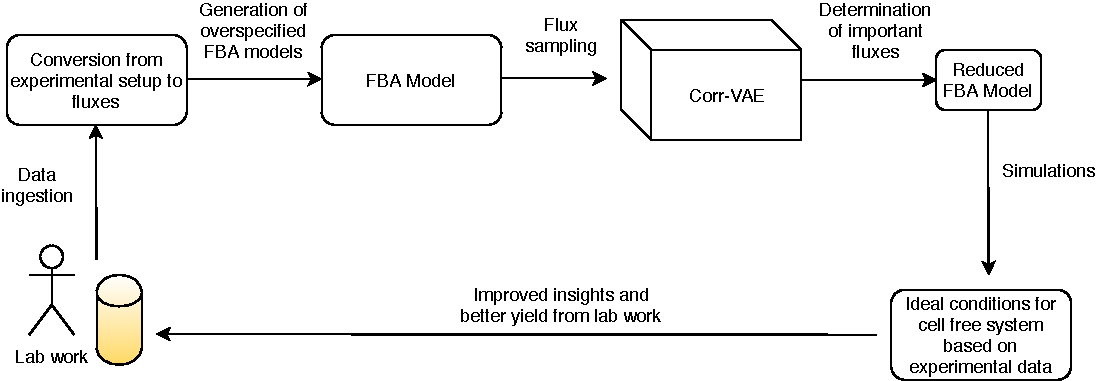
\includegraphics[width=\textwidth]{figs/SystemOverview.pdf}
\end{center}
\caption[The overall pipeline for \gls{sys}]{The overall pipeline for \gls{sys}.
Given an experimental setup and experimental data, \gls{sys} generates a reduced cell-free metabolic model from the corresponding \gls{gem}.}
\label{fig:overview}
\end{figure}

The structure of this dissertation is as follows.
%TODO add back in?
Chapter \ref{chap:bkg} provides background information on cell-free systems, \gls{fba}, and \glspl{vae}.
%We describe the different types of cell-free systems, how we produce our system, and some uses and advantages for cell-free systems.
%Then, we explore the mathematical foundations of \gls{fba} and how it can be used to model biological systems.
%Finally, we explain how autoencoders are used for dimensionality reduction, specifically focusing on how VAEs work.
Chapter \ref{chap:rw} introduces related work in the fields of metabolic models, reduction of metabolic models, modeling cell-free systems, and \glspl{vae}.
%We analyze the current state of the art in metabolic modeling, specifically focusing on the development of \gls{fba} and the creation of a GEM for \ecoli.
%Next, we focus on how search techniques have been used to reduce metabolic models to their core reactions.
%Then, we share efforts to model cell-free systems, describing two prior works that have applied \gls{fba} to cell-free systems.
%Finally, we outline the relevant literature about VAEs.
Chapter \ref{chap:impl} describes \gls{sys}, the system I have built to generate \gls{cfps} models (shown in Figure \ref{fig:overview}).
%We begin by describing our experimental setup and how we generated our data.
%Next, we detail how to ingest the experimental setup and data and convert it into a metabolic model.
%Then, we explain how we used that model to generate a larger dataset for our deep learning algorithms.
%Lastly, we use that dataset to train a VAE, which generates a lower dimensionality representation that can be used to create better cell-free metabolic models.
Chapter \ref{chap:res} examines the results of using a \gls{vae} to reduce \gls{fba} models.
Notably, I show that the reduced models \gls{sys} produces are better at describing \gls{cfps} systems than both \glspl{gem} and already published reduced models.
%We also show novel biological insights that were unearthed due to my system.
%Finally, we illustrate how a model can be learned on one set of biological data and transfer to a different set of data. 
Chapter \ref{chap:fw} discusses future work and provides suggestions of how this work may be utilized.
The final chapter concludes with an overview of the project and its key advances.
